%%%%%%%%%%%%%%%%%%%%%%%%%%%%%%%%%%%%%%%%%
% Beamer Presentation
% LaTeX Template
% Version 1.0 (10/11/12)
%
% This template has been downloaded from:
% http://www.LaTeXTemplates.com
%
% License:
% CC BY-NC-SA 3.0 (http://creativecommons.org/licenses/by-nc-sa/3.0/)
%
%%%%%%%%%%%%%%%%%%%%%%%%%%%%%%%%%%%%%%%%%

%----------------------------------------------------------------------------------------
%	PACKAGES AND THEMES
%----------------------------------------------------------------------------------------

\documentclass{beamer}

\mode<presentation> {

% The Beamer class comes with a number of default slide themes
% which change the colors and layouts of slides. Below this is a list
% of all the themes, uncomment each in turn to see what they look like.

%\usetheme{default}
%\usetheme{AnnArbor}
%\usetheme{Antibes}
%\usetheme{Bergen}
%\usetheme{Berkeley}
%\usetheme{Berlin}
%\usetheme{Boadilla}
%\usetheme{CambridgeUS}
%\usetheme{Copenhagen}
%\usetheme{Darmstadt}
%\usetheme{Dresden}
%\usetheme{Frankfurt}
%\usetheme{Goettingen}
%\usetheme{Hannover}
%\usetheme{Ilmenau}
%\usetheme{JuanLesPins}
%\usetheme{Luebeck}
%\usetheme{Madrid}
%\usetheme{Malmoe}
%\usetheme{Marburg}
%\usetheme{Montpellier}
%\usetheme{PaloAlto}
%\usetheme{Pittsburgh}
%\usetheme{Rochester}
%\usetheme{Singapore}
%\usetheme{Szeged}
\usetheme{Warsaw}

% As well as themes, the Beamer class has a number of color themes
% for any slide theme. Uncomment each of these in turn to see how it
% changes the colors of your current slide theme.

%\usecolortheme{albatross}
%\usecolortheme{beaver}
%\usecolortheme{beetle}
%\usecolortheme{crane}
%\usecolortheme{dolphin}
%\usecolortheme{dove}
%\usecolortheme{fly}
%\usecolortheme{lily}
%\usecolortheme{orchid}
%\usecolortheme{rose}
%\usecolortheme{seagull}
%\usecolortheme{seahorse}
%\usecolortheme{whale}
%\usecolortheme{wolverine}

%\setbeamertemplate{footline} % To remove the footer line in all slides uncomment this line
%\setbeamertemplate{footline}[page number] % To replace the footer line in all slides with a simple slide count uncomment this line

%\setbeamertemplate{navigation symbols}{} % To remove the navigation symbols from the bottom of all slides uncomment this line
}

\usepackage{graphicx} % Allows including images
\usepackage{booktabs} % Allows the use of \toprule, \midrule and \bottomrule in tables

%----------------------------------------------------------------------------------------
%	TITLE PAGE
%----------------------------------------------------------------------------------------

\title[Euler Circuits]{Euler Circuits on DiGraph } % The short title appears at the bottom of every slide, the full title is only on the title page

\author{Nilay Bhatt} % Your name
\institute[CCSU] % Your institution as it will appear on the bottom of every slide, may be shorthand to save space
{
Central Connecticut State University \\ Dr. Rachel Schwell\\ % Your institution for the title page
\medskip
\textit{nilaybhatt@my.ccsu.edu} % Your email address
}
\date{\today} % Date, can be changed to a custom date

\begin{document}

\begin{frame}	
\titlepage % Print the title page as the first slide
\end{frame}

\begin{frame}
\frametitle{Overview} % Table of contents slide, comment this block out to remove it
\tableofcontents % Throughout your presentation, if you choose to use \section{} and \subsection{} commands, these will automatically be printed on this slide as an overview of your presentation
\end{frame}

%----------------------------------------------------------------------------------------
%	PRESENTATION SLIDES
%----------------------------------------------------------------------------------------

%------------------------------------------------
\section{Definitions} 
\begin{frame}
\frametitle{Definitions}
\begin{definition}[Graph]
A \textbf{graph} $G$ consists of a non-empty finite set $V(G)$ of elements called \textbf{vertices},
and a finite `family'  $ E(G)$ of unordered pairs of (not necessarily distinct) elements
of $V(G)$ called \textbf{edges}.
\end{definition}
\begin{itemize}
\item Too formal? Think of a graph as a bunch of tennis balls connected with a thread.
\end{itemize}
\begin{definition}[Digraph]
A \textbf{digraph} $G$ consists of a non-empty finite set $V(G)$ of elements called \textbf{vertices},
and a finite `family'  $E(G)$ of ordered pairs of distinct elements of $V(G)$ called \textbf{directed edges}.
\end{definition}
\begin{itemize}
\item NYC grid with the streets being one-way, which then restricts our direction of movement on the graph.
\end{itemize}
\end{frame}

%------------------------------------------------

%\subsection{Subsection Example} % A subsection can be created just before a set of slides with a common theme to further break down your presentation into chunks

\begin{frame}
\frametitle{Graphs and Digraphs}
\begin{figure}[h]
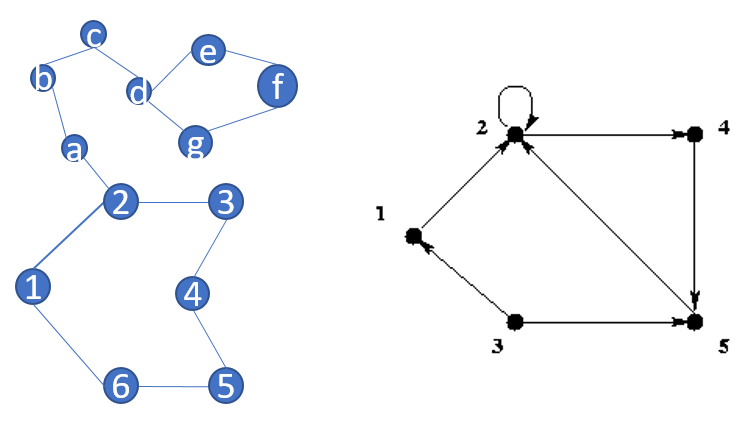
\includegraphics[width=\textwidth]{graphs.png}
\end{figure}
\end{frame}

%------------------------------------------------
\section{Eulerian Graphs}
\begin{frame}
\frametitle{Euler Paths v/s. Circuits}
\begin{definition}[Euler Path]
 An \textbf{Euler path} on a graph $G$ is a special walk that uses each edge exactly once, and it starts and ends at \textbf{different} vertices.
\end{definition}
\begin{definition}[Euler Circuit]
 An \textbf{Euler circuit} on a graph $G$ is a walk that uses each edge exactly once, and it starts and ends at the \textbf{same} vertex.
\end{definition}
\end{frame}

%------------------------------------------------

\begin{frame}
\frametitle{Euler Path}
\begin{figure}[h]
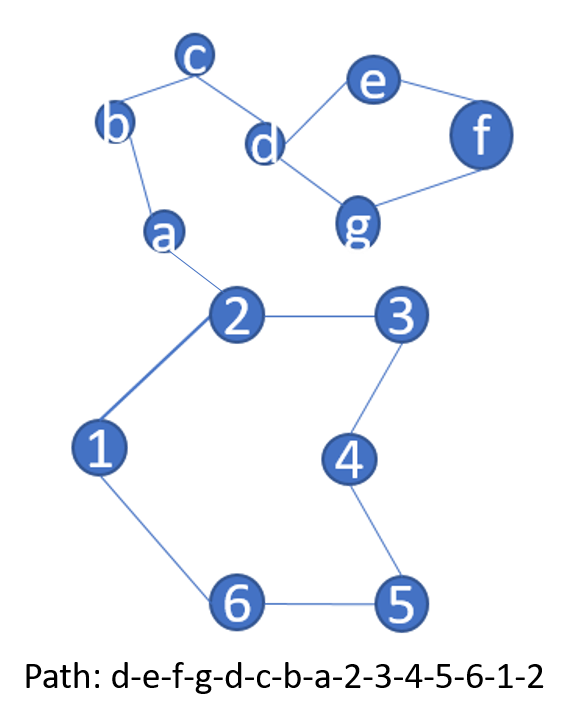
\includegraphics[scale = 0.3]{path.png}
\end{figure}
\end{frame}

%------------------------------------------------


\begin{frame}
\frametitle{Euler Circuit}
\begin{figure}[h]
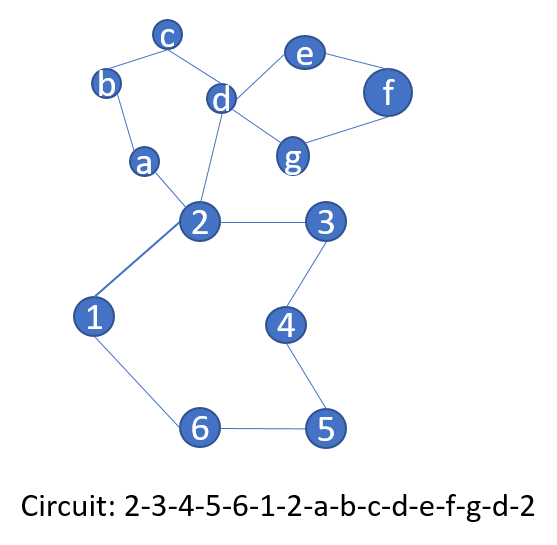
\includegraphics[scale = 0.4]{circuit.png}
\end{figure}
\end{frame}

%------------------------------------------------


\begin{frame}
\frametitle{Criterion for an Euler path or circuit on a given (di)graph}
\begin{block}{Euler Path}
A given \textbf{graph} $G$ has an Euler path if: \textbf{All but 2 vertices in the graph are of odd degree.}\\ A digraph $D_g$ has an Euler path if: the above condition plus \textbf{"the $|indegree - outdegree| = 1$ for given two vertices in $D_g$.}
\end{block}
\pause
\begin{block}{Euler Circuit}
A graph $G$ has and Euler circuit if and only if all the vertices are of \textbf{even degree} and is connected. 
\end{block}
\pause
\begin{itemize}
\item What extra condition do you think will be needed on a digraph?
\end{itemize}
\end{frame}

%------------------------------------------------

\begin{frame}
\frametitle{Criterion for an Euler path or circuit on a given (di)graph}
\begin{block}{Euler Circuit on digraphs}
A graph $G$ has and Euler circuit if and only if all the vertices are of \textbf{even degree} and is connected and \textbf{the indegree = outdegree for all vertices}
\end{block}

\pause
 A theorem with proper proof done for the semester project in \textbf{Seminar in Proof} course.
\end{frame}

%------------------------------------------------

\begin{frame}
\frametitle{How to find an Euler path and/or circuit on a graph?}
\begin{itemize}
\item The graph has to be connected
\pause
\item For an Euler Path there can be either $0$ or $2$ odd degree vertices. For an circuit all of them has to be even. To traverse an Euler path, start at either of the odd vertex.
\pause
\item Follow edges one at a time. If you have a choice between a bridge and a non-bridge, always choose the non-bridge. (If removal of a single edge from a connected graph can make it disconnected then such an edge is called a \textbf{bridge}.)
\end{itemize}
\pause
This is called \textbf{Fleury's Algorithm}
\end{frame}

%------------------------------------------------


\begin{frame}
\frametitle{Find an Euler Path?}
\begin{figure}[h]
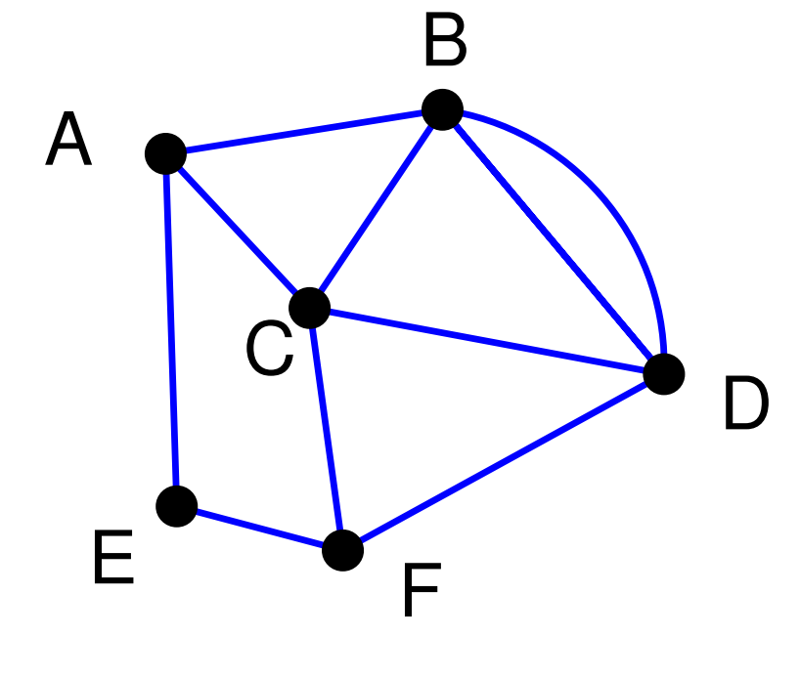
\includegraphics[scale = 0.4]{path2.png}
\end{figure}
\end{frame}

%------------------------------------------------

\begin{frame}
\frametitle{Euler Circuit on digraph}
\begin{figure}[h]
\includegraphics[scale = 0.8]{eulerdi.jpg}
\end{figure}
\end{frame}

%------------------------------------------------

\begin{frame}
\frametitle{What's next?}
This is cool, but for all the applied mathematicians in the room and computer engineers like me the question lies:\\ 
\textbf{\begin{center}
How does that help me?
\end{center}}
\end{frame}

%------------------------------------------------

%------------------------------------------------
%------------------------------------------------
\section{Genome Sequencing}
%------------------------------------------------
%------------------------------------------------

%------------------------------------------------

\begin{frame}
\frametitle{Multiple Columns}
\begin{columns}[c] % The "c" option specifies centered vertical alignment while the "t" option is used for top vertical alignment

\column{.45\textwidth} % Left column and width
\textbf{Heading}
\begin{enumerate}
\item Statement
\item Explanation
\item Example
\end{enumerate}

\column{.5\textwidth} % Right column and width
Lorem ipsum dolor sit amet, consectetur adipiscing elit. Integer lectus nisl, ultricies in feugiat rutrum, porttitor sit amet augue. Aliquam ut tortor mauris. Sed volutpat ante purus, quis accumsan dolor.

\end{columns}
\end{frame}

%------------------------------------------------
\section{Second Section}
%------------------------------------------------

\begin{frame}
\frametitle{Table}
\begin{table}
\begin{tabular}{l l l}
\toprule
\textbf{Treatments} & \textbf{Response 1} & \textbf{Response 2}\\
\midrule
Treatment 1 & 0.0003262 & 0.562 \\
Treatment 2 & 0.0015681 & 0.910 \\
Treatment 3 & 0.0009271 & 0.296 \\
\bottomrule
\end{tabular}
\caption{Table caption}
\end{table}
\end{frame}

%------------------------------------------------

\begin{frame}
\frametitle{Theorem}
\begin{theorem}[Mass--energy equivalence]
$E = mc^2$
\end{theorem}
\end{frame}

%------------------------------------------------

\begin{frame}[fragile] % Need to use the fragile option when verbatim is used in the slide
\frametitle{Verbatim}
\begin{example}[Theorem Slide Code]
\begin{verbatim}
\begin{frame}
\frametitle{Theorem}
\begin{theorem}[Mass--energy equivalence]
$E = mc^2$
\end{theorem}
\end{frame}\end{verbatim}
\end{example}
\end{frame}

%------------------------------------------------

\begin{frame}
\frametitle{Figure}
Uncomment the code on this slide to include your own image from the same directory as the template .TeX file.
%\begin{figure}
%\includegraphics[width=0.8\linewidth]{test}
%\end{figure}
\end{frame}

%------------------------------------------------

\begin{frame}[fragile] % Need to use the fragile option when verbatim is used in the slide
\frametitle{Citation}
An example of the \verb|\cite| command to cite within the presentation:\\~

This statement requires citation \cite{p1}.
\end{frame}

%------------------------------------------------

\begin{frame}
\frametitle{References}
\footnotesize{
\begin{thebibliography}{99} % Beamer does not support BibTeX so references must be inserted manually as below
\bibitem[Smith, 2012]{p1} John Smith (2012)
\newblock Title of the publication
\newblock \emph{Journal Name} 12(3), 45 -- 678.
\end{thebibliography}
}
\end{frame}

%------------------------------------------------

\begin{frame}
\Huge{\centerline{The End}}
\end{frame}

%----------------------------------------------------------------------------------------

\end{document}